
\documentclass[11pt,a4paper]{article}
\usepackage[left=2cm,right=2cm,top=2cm,bottom=3cm]{geometry}
\usepackage{amsmath,amsfonts,amsthm,amssymb,varioref,times, commath}
\usepackage{gensymb}
\usepackage{tikz}
\usepackage{textcomp}
\usepackage{hyperref}
\hypersetup{
 colorlinks=true,
 linkcolor=blue,
 filecolor=magenta, 
urlcolor=cyan,
}
\usepackage{lipsum}
\usepackage{epigraph}
%to resume numbering in a list
\usepackage{enumitem}
%----- arrows 
\usepackage{extarrows}

%    differential equatiosn 
\usepackage{diffcoeff}   %\diff[2]{x}{y}


%%%%%%pour ecrire en français avec les accents
\usepackage[utf8]{inputenc}
\usepackage[T1]{fontenc}
\usepackage{lmodern} % load a font with all the characters
\usepackage{units}
%%%%%%%Image-related packages
\usepackage{wrapfig}
\usepackage{float, graphicx}
\graphicspath{ {./img/} }
\usepackage{subcaption}
\usepackage[export]{adjustbox}

%%%%%%%pour faire des cadres
\usepackage{xcolor}
\usepackage{tcolorbox}
\usepackage{framed}
\usepackage{mdframed}


%%%%%%%chemistry frmulae
\usepackage{chemfig}
\usepackage{chemformula}
\usepackage[version=4]{mhchem}

% -------------- Circuits -------------------
\usepackage[european, straightvoltages]{circuitikz}

% Title & headers
\usepackage[explicit]{titlesec}
% Raised Rule Command:
% Arg 1 (Optional) - How high to raise the rule
% Arg 2 - Thickness of the rule
\newcommand{\raisedrulefill}[2][0ex]{\leaders\hbox{\rule[#1]{1pt}{#2}}\hfill}
\titleformat{\section}{\Large\bfseries}{\thesection. }{0em}{#1\,\raisedrulefill[0.4ex]{1pt}}

% pour ecrire sur +sieurs colonnes
\usepackage{multicol}
\setlength{\columnseprule}{0pt}
\setlength{\columnsep}{60pt}
% Fusion de lignes de tableaux.
\usepackage{multirow}
% Position verticale des lettres dans la ligne de tableau.
\usepackage{array}

% physics -----------------------------------------------------------
\newcommand{\To}{\longrightarrow}
\newcommand{\gpl}{\; g\cdot L^{-1}}
\newcommand{\gpmol}{\; g\cdot mol^{-1}}
\newcommand{\mpl}{\; mol\cdot L^{-1}}
\newcommand{\mps}{\; m\cdot s^{-1}}
\newcommand{\rps}{\; rad\cdot s^{-1}}
\newcommand{\kph}{\; km\cdot h^{-1}}
\newcommand{\mpss}{\; m\cdot s^{-2}}
\newcommand{\Dt}{\Delta t}
\newcommand{\vv}{\vec{v}}
\newcommand{\va}{\vec{a}}
\newcommand{\vp}{\vec{p}}
\newcommand{\vf}{\vec{F}}
\newcommand*{\Vf}[1]{\overrightarrow{F_\ensuremath{{#1}}}}
\newcommand{\es}[1]{\cdot10^{#1}}
\newcommand{\eng}[1]{\textcolor{purple}{(= #1})}
\usepackage{harpoon}
%\newcommand*{\vect}[1]{\overrightharp{\ensuremath{#1}}}
\newcommand*{\Vect}[1]{\overrightarrow{\ensuremath{#1}}}
\newcommand{\pfd}[1]{\sum \vec{F}_{ext_{#1}} &= \od{\vp_{#1}}{t} = m\cdot\va_{#1}}
\newcommand{\C}{\degree C}
\newcommand{\Delt}{\Delta t}

% --- Circuits ------------
\newcommand{\bipole}[1]{
\begin{circuitikz} \draw
(0,0) to[ #1 ] (2,0); 
\end{circuitikz} {\hspace{5mm}}}

% Chimie ---------------------------------
\newcommand{\oxo}{\ce{H3O+}_{(aq)}}
\newcommand{\eau}{\ce{H2O}_{(\ell)}}
\newcommand{\OH}{\ce{HO-}_{(aq)}}
\newcommand{\AH}{\ce{AH}_{(aq)}}
\newcommand{\A}{\ce{A-}_{(aq)}}
\newcommand{\MnO}{\ce{MnO_4^{-}}}
\newcommand{\conc}[1]{\left[{#1}\right]}
\newcommand{\couple}[2]{\ce{#1/#2}}


% Environnements ------------------------
\newcounter{exo}
\newenvironment{exo}[1][]
{\refstepcounter{exo} \begin{shaded}\noindent $\triangleright \quad$\textbf{Exercice~\theexo. #1} } { \end{shaded}}
\newenvironment{eg}
{\begin{shaded} \textbf{Exemple:} } { \end{shaded}}

\newenvironment{defn}[1]
{\begin{leftbar}\noindent \textbf{Définition :\textit{ \quad #1}} } { \end{leftbar}}

%\newenvironment{rmrq}
%{\begin{shaded} \textbf{Remarque.\quad } \itshape } { \end{shaded}}
\newenvironment{rmrq}
{\begin{mdframed}[backgroundcolor=blue!10, linewidth=0pt] \textbf{Remarque.\quad } \itshape } { \end{mdframed}}

\newenvironment{python}
{\begin{shaded} \textbf{A faire en PYTHON}\\ \itshape } { \end{shaded}}

% Shading colour -----------------------------
\definecolor{shadecolor}{gray}{0.9}

\date{}
\author{}

\renewcommand*\contentsname{Résumé}









% Title & headers 
\usepackage{fancyhdr}
\pagestyle{fancy}
\fancyhf{}
\lhead{SciPhy : Terminale spé}
\rhead{Ch. 4 : Thermodynamique}
\chead{2020-28}
\rfoot{Page \thepage}
\lfoot{\textcopyright\; S Zayyani}
\renewcommand{\footrulewidth}{0.1pt}% default is 0pt

\title{\large Physique - Chapitre 4 \\ \LARGE  La Thermodynamique}
\date{}
\author{}

\setlength{\parindent}{0mm}
\setlength{\parskip}{2mm}

%%%%%%%%%%% For wrapfigure
%\setlength{\intextsep}{6pt}%
%\setlength{\columnsep}{3pt}%

\setlength{\columnsep}{15pt}%
\setlength{\intextsep}{-10pt}%


\begin{document}
\maketitle
\vspace{-1cm}
\begin{tcolorbox}[title=Notions de la classe de première à rappeler]
calcul d'une dérivé ; loi de Mariotte ; travail ; Loi de Wien
%\tcblower
\end{tcolorbox}
\tableofcontents

\section{Systèmes thermiques}

La \textbf{thermodynamique} est un vaste branche de la physique concernée par des phénomènes en lien avec les échanges thermiques, la température des systèmes, etc. Aujourd'hui l'étude des phénomènes thermodynamique à l'échelle atomique s'appelle la mécanique statistique, car finalement les phénomènes thermodynamique macroscopique peuvent être expliqués grâce à l'étude du comportement d'un système composé d'un très grand nombre d'entités microscopiques. 

\begin{defn}{Système thermique}
\begin{itemize}
    \item Un \textbf{ensemble} de $N$ entité microscopique, dans un volume donné. 
    \item Tout ce qui n'est pas dans le système est considéré comme l'\textbf{extérieur}. 
    \item Un système thermique est caractérisé par des \textbf{variables d'état}, qui peuvent être des variable macroscopiques ou microscopiques. 
\end{itemize}
\end{defn}

\subsection{Les variables d'état}
Les variable d'états sont des grandeurs physiques qui caractérisent un système thermique. Voici les plus importantes :  

\begin{itemize}
    \item \textbf{Température $T$ : } Une mesure de l'agitation thermique du système, C'est-à-dire une mesure de l'énergie cinétique moyenne des particules constituant le système. L'unité légale de la température est le \textbf{kelvin} $(K)$. 
    \item \textbf{Pression $P$ :} Une mesure de la force exercée par le système thermique sur les parois de son récipient. A l'échelle microscopique, il s'agit d'une mesure de la force, et du nombre de choc des particules du système sur une surface plane. 
    \item \textbf{Masse $M$ :} Une mesure de la masse totale des particules constituant le système. L'unité légale de la masse est le kilogramme $kg$.
    \item \textbf{Volume $V$ :} Une mesure de la place prise pour le système thermique. L'unité légale du volume est le mètre cube $m^3$.
    \item \textbf{Masse volumique $\rho$ : } Une mesure de la masse du système pour un volume donné. L'unité légal est le $kg\cdot mol^{-1}$ 
\end{itemize}

\subsection{Grandeurs intensive \& extensive}

Les grandeurs thermodynamiques (et physique en général), sont divisées en deux catégories : 
\begin{itemize}
    \item \textbf{Grandeurs intensives :} Les grandeurs physiques qui ne dépendent pas de la 'taille` du système. La température et la pression sont deux grandeurs intensives. 
    \item \textbf{Grandeurs extensives :} Les grandeurs physiques dont la valeur dépend de la taille du système; il s'agit donc des grandeurs qui sont proportionnelles à une quantité du système. La masse et le volume sont deux grandeurs extensives. 
\end{itemize}

\subsection{Équilibre d'un système thermique}

La notion d'équilibre en physique est fondamentale, et à l'origine de l'explication d'un très grand nombre de phénomènes des branches diverse de la physique. 

\textbf{En général, l'état d'équilibre est l'état final vers lequel tout système tend, avec le temps}. C'est un état de \textbf{stabilité} maximum, où il règne une sorte de symétrie dans les paramètres du système. 

Dans le cadre thermodynamique, l'équilibre est l'état vers lequel vont tendre deux systèmes thermiques en contact avec des paramètres d'état différents (températures différents). Nous verrons l'application de cela plus tard, dans le cadre des transferts thermiques. 

\section{Le modèle du `Gaz Parfait'}

Un gaz parfait \eng{ideal gas} est le nom donné au modèle thermodynamique (empirique) des gaz réels à basse pression. 

C'est un modèle qui date surtout du $XIX^e$ siècle, où il prend sa forme finale, que l'on utilise aujourd'hui. 

C'est un modèle simplifié, qui s'applique à la plupart des gaz réels à basse température, indépendemment de leur nature (molécule, masse molaire, etc), permettant une caractérisation de leur comportement en fonction, simplement, des leurs variables d'état. C'est-à-dire tous les gaz, comme le dioxygène, méthane ou le diazote se comportent exactement de la même manière, dans la limite du modèle. 

\subsection{L'équation d'état}

Le modèle du gaz parfait, et les différentes lois disparates décrivant le comportement des gaz parfaits (c.f. ci-après) ont finalement était réuni (par Emile Clapeyron, ingénieur et physicien français) sous forme de la \textbf{loi des gaz parfaits} \eng{ideal gas law}. 

\begin{defn}{L'équation d'état des gaz parfaits}
\begin{itemize}
    \item La loi des gaz parfait est l'\textbf{équation d'état} des gaz parfaits
    \item Cette loi s'écrit : 
    \[  PV = nRT \quad \quad \text{où}\quad \quad 
    \begin{cases}
    P \rightarrow \text{la pression du gaz en }(Pa) \\
    V \rightarrow \text{volume du gaz en }(m^3) \\ 
    n \rightarrow \text{la quantité de gaz en }(mol) \\
    T \rightarrow \text{la température du gaz en }(K) \\
    \end{cases}
    \]
    \item $R$ est la \textbf{constante des gaz parfaits}\eng{Ideal/universal gas constant}, et a pour valeur $R = 8,314\;J\cdot K^{-1}\cdot mol^{-1}$
\end{itemize}
\end{defn}
Il y a différentes façons de comprendre cette loi. Dans un premier temps il s'agit d'un point culminant des différentes lois concernant des gaz, qui sont, finalement, chacune un cas particulier de la loi des gaz parfaits : 
\begin{itemize}
    \item \textbf{Loi de Boyle-Mariotte : } $PV = P'V' = K(T,n) $ 
    \item \textbf{Loi de Charles : }  $\frac{V}{T}=\frac{V'}{T'} = K(P,n) $
    \item \textbf{Loi de Gay-Lussac : } $\frac{P}{T}=\frac{P'}{T'} = K(V,n) $
    \item \textbf{Loi d'Avogadro :} $\frac{V}{n}=\frac{V'}{n'} = K(P,T) $
\end{itemize}

Sinon, nous pouvons y arriver par un raisonnement moins empirique, considérant les différents facteurs influençant la pression d'un gaz dans un récipient fermé : 
\[ 
\begin{cases}
     P\propto T \\
     P \propto n \\ 
     P \propto \dfrac{1}{V}
\end{cases}
\Leftrightarrow
     P\propto \dfrac{n\cdot T}{V}
\]

Et donc, pour passer d'une proportionnalité à une égalité, on introduit une constante de proportionnalité, ici $ R $ la constante des gaz parfait, et nous arrivons à la loi des gaz parfaits. 

\begin{exo}
Montrer l'équivalence de la loi des gaz parfait et la relation $n=\dfrac{V}{V_m}$ où $V_m$ est le volume molaire d'un gaz parfait. 
\vspace{2cm}
\end{exo}

\begin{exo}
Montrer l'équivalence de la loi des gaz parfaits et les lois de Boyle-Mariotte, de Charles, de Gay-Lussace et d'Avogardo. 
\vspace{4cm}
\end{exo}


\begin{rmrq}
La loi des gaz parfaits est applicable dans la limite des pression basses, et l'absence de toute interactions entre les particules constituant le gaz. 
\end{rmrq}


\section{Principes de la thermodynamique}

\begin{quote}
    « Au cours d'une transformation quelconque d'un système fermé, la variation de son énergie est égale à la quantité d'énergie échangée avec le milieu extérieur, par transfert thermique (chaleur) et transfert mécanique (travail). »
\end{quote}

Avant de décortiquer cet énoncé, réfléchissons de nouveau à la notion de \textit{travail}. On a vu que la notion de travail est centrale en physique.  Le travail effectué par une force peut avoir deux conséquences importantes :
\begin{itemize}
    \item \textbf{Augmenter (ou diminuer) l’énergie cinétique} d’un solide (e.g. un objet en chute libre accélère vers le sol, à cause du travail moteur de son poids ; la vitesse d’une voiture diminue quand elle freine, à cause du travail résistant des freins.) 
    \item \textbf{Augmenter (ou diminuer) l’énergie potentielle} de pesanteur (e.g. la force de nos muscles effectue du travail lors d’une montée en augmentant notre énergie potentielle de pesanteur)
\end{itemize}

Mais, sont-ils les seuls effets possibles  du travail? (bien sur que non, sinon je n'aurais pas posé la question!)  Étudions donc quelques situations différentes :

\begin{wrapfigure}{l}{0.5\textwidth}
  \centering
  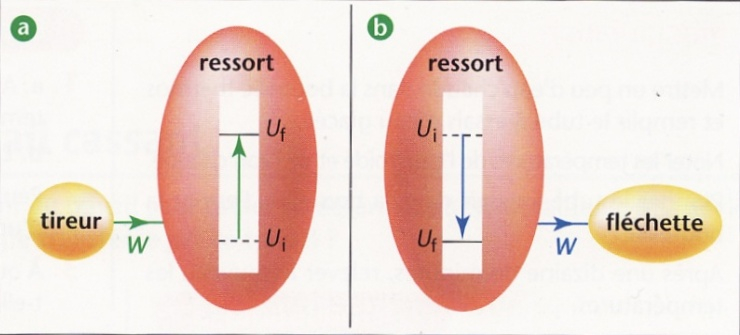
\includegraphics[width=.95\linewidth]{imgs/p4/ressort2.jpg}
\end{wrapfigure}

$\blacktriangleright$ \textbf{Déformation d'un ressort : }
Nous avons déjà vu que l’application d’une force peut entraîner la déformation d’un solide.  Certains matériaux reprennent leur forme originale dans l’absence des forces extérieures : il s’agit de matières élastiques dont un ressort est l’exemple classique.  Étudions alors  le comportement d’un ressort :
\begin{itemize}
    \item La compression d’un ressort nécessite l’application d’une force, qui déplace une partie du ressort.  La force effectue du travail en déformant – élastiquement – le ressort.
    \item La disparition de la force permet au ressort de revenir à sa forme originale, où il exerce une force sur d’autres corps attachés ou en contact avec le ressort
\end{itemize}
\textbf{Interprétation : } Une force travaille en provoquant une déformation élastique.  Ce travail est alors un transfert d’énergie  vers le corps élastique.  Cette énergie est alors « stockée » dans le corps élastique.  En reprenant sa forme originale il peut à son tour restituer de l’énergie en exerçant des forces qui travaillent.  

\begin{wrapfigure}{r}{0.3\textwidth}
  \centering
  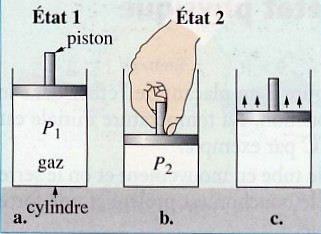
\includegraphics[width=.95\linewidth]{imgs/p4/pression.jpg}
\end{wrapfigure}

$\blacktriangleright$ \textbf{Changement de pression : }

Un gaz (parfait) peut se comporter comme un ressort. Imaginons un gaz à l’état initial, un tel gaz dans un piston de volume $V$.  En appuyant sur le piston, une force s’exerce sur le gaz qui a pour effet la compression de ce dernier : elle a effectué du travail (en déplaçant le piston).  Dans ce état ‘final’ le gaz a un nouveau volume $V$’.  Si la force se relâche, le gaz va se détendre en poussant et re-déplaçant le piston vers l’état initial.  

\begin{wrapfigure}{l}{0.3\textwidth}
  \centering
  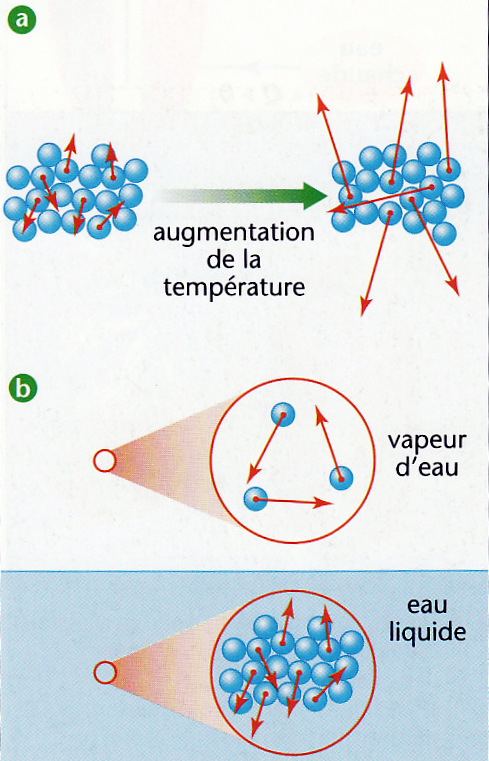
\includegraphics[width=.95\linewidth]{imgs/p4/changetat.jpg}
\end{wrapfigure}

$\blacktriangleright$ \textbf{Changement de température : }

En frottant deux bouts de bois on peut les mettre en feu.  Une autre manière d’observer ce phénomène est l’expérience de Tyndall, où on peut montrer que la température d’un liquide augmente en fonction de la « quantité de frottement » subite par le système.  

\textbf{Interprétation : } Dans les deux cas la force exercée (pendant le frottement) transfert de l’énergie – via le travail effectué – vers le corps frotté.  Cette énergie transférée fait monter la température du liquide.  Cette croissance de la température signifie une augmentation de la vitesse des particules constituant le liquide, c'est-à-dire leur énergie cinétique.

$\blacktriangleright$ \textbf{Changement d'état physique : }

Une force qui travaille peut également provoquer un changement d’état (par exemple du à l’augmentation de la température).  Encore une fois, l’énergie transférée par le travail de la force sert à augmenter l’énergie cinétique des particules.  Cela se manifeste à l’échelle macroscopique comme un changement de température, qui provoque un changement d’état. 

\subsection{Énergie interne d'un système}
Dans tous les cas précédents le travail a transféré de l’énergie vers le corps qui subit le travail.  Cette énergie est par la suite stockée par le corps, sous forme d’une nouvelle forme d’énergie : \textbf{Énergie Interne}.

\begin{defn}{Énergie Interne }\eng{Internal energy}
\begin{itemize}
    \item L’énergie interne d’un système, notée $U$, est l’\textbf{énergie stockée} par ce système, autrement que sous forme d’énergie cinétique ou potentielle de pesanteur.  Comme toutes formes d’énergie, elle s’exprime en Joules ($J$).
    \item Énergie interne d’un système macroscopique résulte de \textbf{contributions microscopiques} : l’énergie cinétique microscopique et l’énergie potentielle microscopique. 
    \item L’énergie interne est la somme des énergies internes des constituants du système : 
    \[ U_{AB} = U_A + U_B   \]
\end{itemize}
\end{defn}

Nous pouvons définir aussi l'énergie totale d'un système qui serait la somme de son énergie mécanique et son énergie interne : $E_{tot} = E_m + U = E_c + E_p + U$

\begin{rmrq}
Il est important de comprendre que l’énergie interne d’un système regroupe les énergies cinétiques et potentielles des particules qui les constituent au niveau \textbf{microscopique}.  C'est-à-dire \textbf{l’énergie interne est une grandeur macroscopique provenant (émergeant) du comportement microscopique des constituants de la matière}.  Voici quelques exemples de ce phénomène :
\begin{itemize}
    \item la grandeur macroscopique \textbf{Température} qui n’est qu’une mesure macroscopique de l’énergie cinétique des particules à l’échelle microscopique.
    \item la \textbf{pression} n’est qu’une manifestation macroscopique des forces exercées par les chocs microscopiques entre les particules et la paroi du récipient.
    \item La \textbf{déformation élastique} modifie des distances entre les particules, et donc les interactions entre ces particules (eg. Interactions coulombiennes, etc.)
\end{itemize}
\end{rmrq}

\subsection{Premier principe de la thermodynamique}

Un dernier mot avant de continuer vers le premier principe de thermodynamique: (comme c'est souvent le cas en physique,) ce qui est plus significatif que l'énergie interne d'un système, est la \textbf{variation de l'énergie interne} du système $\Delta U$. 

La variation d’énergie interne $\Delta U$ d’un système est la conséquence d’échanges d’énergie avec l’extérieur par travail $W$, ou par transfert thermique $Q$ . 

\begin{defn}{Premier principe de thermodynamique}
\begin{itemize}
    \item La variation de l'énergie interne d'un système fermé (et de composition fixe) vérifie : 
\[  \Delta U = W + Q   \quad \text{où} \quad 
\begin{cases}
    \Delta U \rightarrow \text{énergie interne en }(J) \\
    W \rightarrow \text{énergie transférée par travail en }(J) \\ 
    Q \rightarrow \text{énergie transférée par transfert thermique en }(J)
\end{cases}\]
    \item Par convention, le travail et le transfert thermique sont comptés \textbf{positivement s’ils sont reçus} par le système et \textbf{négativement s’ils sont cédés} par le système. 
\end{itemize}
\end{defn}

\begin{eg}
Réinterprétons donc le cas de la déformation d'un ressort dans le début de la partie 3, avec le langage du premier principe de thermodynamique. 

De l'énergie est transférée vers le système ($W > 0 $) depuis l'extérieur, grâce au travail d'une force extérieure .  Cette énergie est alors « stockée » dans le corps élastique, augmentant l'énergie interne.  

En reprenant sa forme originale il peut à son tour restituer de l’énergie en exerçant des forces qui travaillent. Ce le système alors qui cède de l'énergie vers l'extérieur, par le billet du travail qu'il effectue sur ce dernier ($W > 0 $).
\end{eg}

\subsection{Capacité thermique}	
Dans le cas d'un système incompressible (comme un liquide ou un solide), il y a un moyen d'établir une relation entre la variation de l'énergie interne et la variation de la température du système. Ceci dépend d'une nouvelle caractéristique du système : la capacité thermique. 

\begin{defn}{Capacité thermique \& capacité thermique massique}
\begin{itemize}
    \item La \textbf{capacité thermique}\eng{heat capacity} $C$ d'une corps est l’énergie thermique que doit recevoir ce corp pour élever sa température d’un degré Celsius, ou d’un kelvin, et vérifie la relation suivante : 
    \[        
    \Delta U = C\dot \left(T_f - T_i\right) = C\cdot\Delta T \; \; où\;\;
    \begin{cases}
    C \rightarrow \text{capacité thermique en }(J\cdot K^{-1}) \\
    \Delta T \rightarrow \text{variation de température en }(K \; ou \; \degree C) \\ 
    \end{cases}
    \]
    \item $C$ est une grandeur \textbf{positive}, et \textbf{extensive}. Il s'agit d'une mesure d'un corps de stocker de l'énergie pour élever sa température. 
    \item La grandeur \textbf{intensive} correspondant, est la \textbf{capacité thermique massique}\eng{specific heat capacity} $c$, donnée par la relation : 
    \[ \Delta U = mc\left(T_f - T_i\right) = m\cdot c\cdot\Delta T \; \; où\;\;
    \begin{cases}
    c \rightarrow \text{capacité thermique massique en }(J\cdot kg^{-1}\cdot K^{-1}) \\
    \Delta T \rightarrow \text{variation de température en }(K \; ou \; \degree C) \\ 
    m \rightarrow \text{masse du système en }(kg ) \\
    \end{cases}       \]
    \item La capacité thermique et la capacité thermique massique sont liées par la masse du système : $c = \dfrac{C}{m}$
\end{itemize}
\end{defn}

La capacité thermique massique étant une grandeur intensive, est une caractéristique de la substance. C'est une mesure de l'énergie nécessaire pour augmenter la température d'un kilogramme d'une substance de $1\degree C$ (indépendemment de la température initiale). Voici un tableau comparant les valeurs de $c$ de différentes substances : 

\begin{figure}[h]
    \centering
    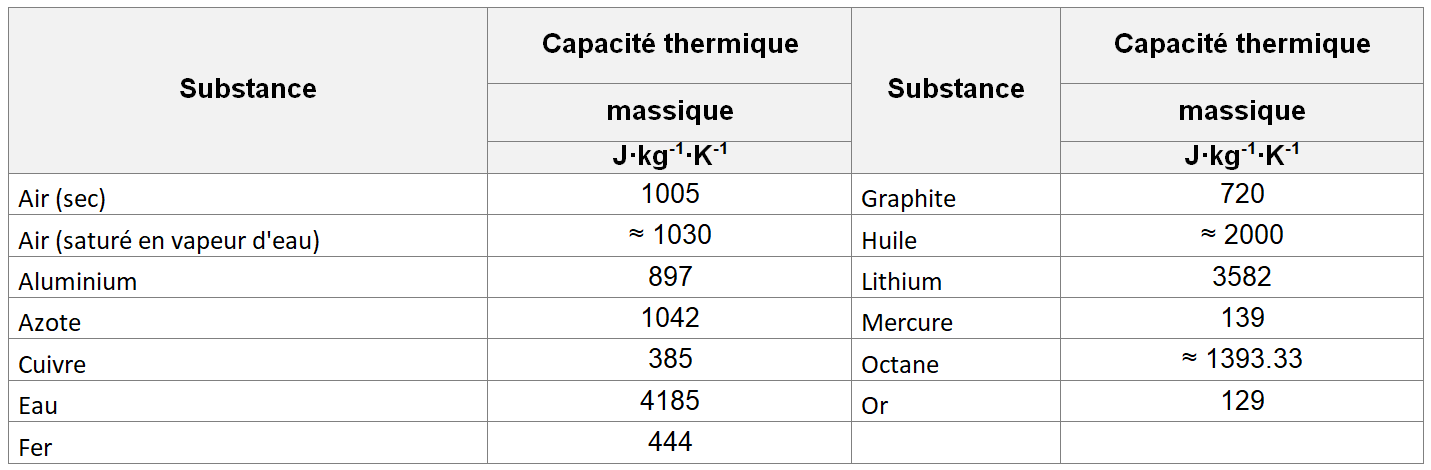
\includegraphics[width=\linewidth]{imgs/p4/tableC.png}
    \caption{les valeurs de $c$ de différentes substances }
    \label{fig:capacités}
\end{figure}

\begin{exo}
Calculer l’énergie nécessaire pour faire monter la température de $1\;kg$ de l’eau de $1\degree C$.
\vspace{3cm}
\end{exo}

\begin{exo}
Calculer l’énergie nécessaire pour faire bouillir $500\; mL$ de l’eau du robinet $(T=20\degree C)$.  
\vspace{4cm}
\end{exo}

\begin{exo}
En se servant des données dans le tableau ci-dessus, quelle hypothèse peut-on avancer pour expliquer pourquoi des métaux comme Fer, Or, ou cuivre sont considérés comme de bons conducteurs thermiques. 
\vspace{4cm}
\end{exo}

\subsection{Les autres principes de la thermodynamique}

\section{Les transferts thermiques}

En tant que bons scientifiques on commence notre investigation avec quelques  questions simples mais importantes :
\begin{enumerate}
    \item Pourquoi quand on laisse du thé chaud sur la table dans une pièce à la température ambiante, au bout de quelques minutes, le thé se refroidit suffisamment pour être buvable ?
    \item Pourquoi une petite cuillère mise dans le thé devient très chaude rapidement ?
    \item Pourquoi a-t-on besoin d’utiliser un Thermos afin de garder notre thé chaud pendant quelques heures ?
    
    Et maintenant quelques questions qui concernent autre chose que du thé.
    \item Pourquoi a-t-on froid en sortant du bain, ou d’une piscine ?
    \item Pourquoi, en hiver,  l’air chaud d’une pièce sort en ouvrant la fenêtre ?
\end{enumerate}

Toutes les situations évoquées ci-dessus sont les exemples du phénomène de transfert thermique. 

\begin{defn}{Transfert thermique}
\begin{itemize}
    \item Un transfert thermique est le transfert d’énergie qui s’effectue entre \textbf{deux corps qui n’ont pas la même température}, (i.e. deux corps qui ne sont pas en équilibre thermique). 
    \item A l’échelle macroscopique, ce déséquilibre se manifeste sous forme d’une différence de température.  Un transfert thermique a donc seulement lieu entre des corps de températures différentes.  
    \item Un transfert thermique s’appelle souvent « chaleur », et est noté par $Q$.
    \item Grâce à ce principe, on peut donc déterminer le sens d’un transfert thermique. Un transfert thermique entre deux corps se produit du corps le plus chaud vers le corps le plus froid. Le transfert cesse lorsque les corps sont à la même température (i.e. quand ils atteignent l’équilibre thermique).  
\end{itemize}
\end{defn} 

\begin{rmrq}
Un des principes fondamentaux de la physique est le principe (ou la recherche) de l’équilibre.  Dans la nature les transferts s’effectuent afin d’établir un équilibre entre les corps en contact/interaction.  Un transfert thermique a donc lieu afin d’équilibrer les énergies thermiques des corps en contact. Le transfert thermique s'arrête une fois cet équilibre atteint, C'est-à-dire une fois les deux corps sont à la même température.
\end{rmrq}

Il existe trois mécanisme de transferts thermique, que l'on aborde en détail par la suite: 
\begin{itemize}
    \item \textbf{Conduction : }Principalement en milieu solide. 
    \item \textbf{Convection : }Principalement en milieu fluide. 
    \item \textbf{Rayonnement (radiation) : }En tout milieu, mais aussi en absence de milieu matériel. 
\end{itemize}

\subsection{Conduction}



La \textbf{conduction thermique} (ou diffusion thermique) est un mode de phénomène de transfert thermique provoqué par une différence de température entre deux régions d'un même milieu, ou entre deux milieux en contact, et se réalisant sans déplacement global de matière. Elle peut s'interpréter comme la \textbf{transmission de proche en proche de l'agitation thermique} : un atome (ou une molécule) cède une partie de son énergie cinétique à l'atome voisin.

Dans un gaz ou un liquide, l'énergie se propage par contact direct entre les molécules au gré des chocs aléatoires à l'échelle microscopique. Dans un solide ou fluide immobilisé, la vibration des atomes autour de leur position d'équilibre dans le solide, se transmet de proche en proche. Les cristaux disposent d'un mode de transfert thermique supplémentaire particulier associé aux vibrations du réseau.

De plus, comme pour l’électricité, on peut avoir des conducteurs thermiques, ainsi que des isolants thermiques.  En fait, maintenant que l’on a compris que la transmission de l’agitation thermique se fait par l’intermédiaire des électrons ainsi que des particules constituant la matière, ce n’est plus surprenant que les meilleurs conducteurs thermiques (métaux)  soient aussi les meilleurs conducteurs électriques. 

\begin{defn}{Flux thermique}
\begin{itemize}
    \item Le flux thermique $\varphi$, appelé aussi la puissance thermique $P_{th}$, est l’énergie transférée à travers une paroi par unité de temps, exprimée : 
\[ \varphi = \dfrac{Q}{\Delta t}   \quad \text{où} \quad
\begin{cases}
    Q \rightarrow \text{énergie thermique transférée en }(J) \\
    \Delta t \rightarrow \text{durée du transfert en }(s) \\ 
\end{cases}
\]
    \item $\varphi$ s’exprime en watts $W$.
\end{itemize}
\end{defn}

\begin{defn}{Résistance thermique}
\begin{itemize}
    \item La résistance thermique (de conduction) $R_{th}$   est une mesure de la résistance d’une substance à un flux thermique. 
    \item La \textbf{résistance thermique} de conduction s'exprime en fonction du flux de chaleur entre deux surfaces isothermes et les températures de ces deux surfaces isothermes (i.e. dont la température est constante)
    \[ R_{th} = \dfrac{T_c - T_f}{\varphi}      
    \quad \text{où} \quad 
    \begin{cases}
    T_c \rightarrow \text{température du corps chaud en }(K \;\text{ou}\;\degree C) \\
    T_f \rightarrow \text{température du corps froid en }(K \;\text{ou}\;\degree C) \\
    \end{cases}
    \]
    \item La résistance thermique s’exprime en $K\cdot W^{-1}$
\end{itemize}
\end{defn}    

Pour un même écart de température donc entre les deux faces d’une paroi, plus la résistance thermique de la paroi est grande et plus le flux thermique est faible. Une paroi de grande résistance thermique est un bon isolant thermique.
\newpage
\begin{exo}
Il faut 3 minutes pour faire chauffer $200\; g $ d'eau du robinet, à $20\C$ initialement à l'ébullition. Déterminer le flux thermique : 
\vspace{5cm}
\end{exo}

\begin{exo}
La température à l'extérieure d'une maison est de $3\degree C$, et à l'intérieur il fait $20\C$ à minuit. Si les parois de la maison présente une réistance thermique de $R_{th} = 1,00\es{-2}\; K\cdot W^{-1}$, déterminer le flux thermique à travers cette paroi. 
\vspace{5cm}
\end{exo}	
	
\subsection{Convection : Loi de Newton}
La convection thermique est le  transfert d'énergie qui s'accompagne de mouvement de molécules dans un fluide (liquide ou gaz). Exemples de transfert par convection : échange de chaleur dans des radiateurs à circulation d'eau ou d'air (convection forcée), refroidissement d'une tasse de liquide chaud en soufflant dessus (convection forcée), diffusion de l'air chaud au-dessus d'un radiateur électrique (convection naturelle s'il n'y a pas de soufflerie dans le radiateur). C'est Newton qui donne une première modélisation de l'évolution de la température d'un corps, son refroidissement, par convection. 

\begin{defn}{Loi de refroidissement de Newton}

Pour un corps à température $T(t)$ dans un environnement thermostat (température constante) à $T_{th}$, l'évolution de la température est décrite par : 
    \[  \varphi = h\cdot S\big(T_{th} - T(t)\big) 
    \quad \text{où} \quad 
    \begin{cases}
    S\rightarrow \text{Surface d'échange en }(m^2) \\
    h\rightarrow \text{coefficient de transfert thermique en }(W\cdot K^{-1}\cdot m^{-2}) \\ 
     \end{cases}
    \]
\end{defn}

\begin{wraptable}{r}{0.35\linewidth}
\begin{rmrq}
\small{Le coefficient de transfert thermique $h$ est comme la propriété inverse de la résistance thermique, que nous avons vu précédemment. Il y a même des points d'analogie entre les propriétés de la conductivité thermique et la conductivité électrique: la résistance thermique étant l'analog de la résistance ohmique, et le coefficient de transfert thermique étant l'analog de la conductance; avec les mêmes règles d'associations valables pour les deux classes de grandeurs. 

De plus, la détermination de sa valeur dépend de la nature du liquide, ainsi que le solide en contact. Il peuvent être déterminés empiriquement, mais aussi par calcul (plutôt compliqué) tenant compte des divers facteurs comme la vitesse des fluides, leurs viscosités, etc.}
\end{rmrq}
\end{wraptable}
\newpage
Voyons alors, si l'on ne peut pas concocter quelques chose d'intéressant en revenant sur la définition du flux thermique, développée précédemment : 

Dans un système ou la seule variation de l'énergie interne est due aux transferts thermiques : $\Delta U = Q = C\Delta T$. Alors : 
\begin{align*}
    \dfrac{Q}{\Delt} &= \dfrac{C\Delta T}{\Delt} \\
    \varphi &= C\dfrac{\big(T(t+\Delt) - T(t) \big)}{\Delt} \\
\end{align*}
Nous reconnaissons alors l'expression du taux d'accroissement, et donc : 
\[  \varphi &= C\od{T}{t} = \od{U}{t}      \]
et en faisant l'équivalence avec la loi de Newton : 
\begin{align*}
    \varphi &= \od{U}{t} = C\od{T}{t} \\
    C\od{T}{t} &= h\cdot S\big(T_{th} - T(t)\big)
\end{align*}
Nous avons alors une équation différentielle de premier ordre, que l'on peut réécrire sous une forme plus canonique : 
\[ \od{T}{t} + \frac{hS}{C}T =  \frac{hS}{C}T_{th}   \]

Comme vous le savez déjà, ayant les conditions initiales (C'est-à-dire $T(t_0) = T_0$ la solution de cette équation est une fonction exponentielle : 
\[ T(t) = T_{th} +\big( T_0 - T_{th} \big)e^{-\nicefrac{t}{\tau}}   \]

avec $\tau = \frac{C}{hS}$, la \textbf{constante du temps}, caractérisant la vitesse d'évolution de température du corps. 

\begin{rmrq}
Nous voyons, encore, une relation différentielle d'ordre 1 (comme dans nos études des vitesses de réaction). Il est important de comprendre que toute grandeur physique dont la variation dépend de valeur de la grandeur, obéira à une relation de ce type. C'est bien le cas ici : le vitesse de refroidissement (i.e. taux de variation de la température $\od{T}{t}$) dépend de la température instantanée du corps qui le subit (i.e. $T(t)$), ou plus précisément la différence entre la température du corps et de son environnement (i.e. $T(t) - T_{th}$). 
\end{rmrq}


\begin{exo}{Démonstration}

Montrer que  $C\od{T}{t} + hST =  hS T_{th}$ a bien pour solution, la fonction exponentielle ci-avant. 
\vspace{4cm}
\end{exo}

\begin{exo}
Du thé chaud, dans une tasse de rayon $4\; cm$ et de hauteur de $10\; cm$, à une température initiale de $85\C$, est placé dans un environnement à une température de $25\C$. Au bout de 5 minutes, il est à $60\C$. 
\begin{enumerate}
    \item Déterminer la température de l'eau au bout de 10 minutes. 
    \item Déterminer la température de l'eau au bout de 20 minutes. 
    \item Au bout de combien de temps peut-on dire que l'eau est en équilibre thermique avec son environnement? 
    \item Déterminer le coefficient de transfert thermique. 
\end{enumerate}
\vspace{10cm}
\end{exo}

\subsection{Rayonnement : Loi de Stefan-Boltzmann}

\subsubsection{Corps noirs}

En physique, un \textbf{corps noir}\eng{black body} signifie un objet idéal qui absorbe parfaitement toute l'énergie électromagnétique (toute la lumière quelle que soit sa longueur d'onde) qu'il reçoit. Ayant absorbé cette radiation, l'agitation thermique qui en résulte, provoque l'émission d'un rayonnement thermique, dit rayonnement du corps noir \eng{black-body radiation}. En contraste, un corps blanc serait un corps réfléchissant tout rayonnement incident, et donc qui n'absorbe rien et n'émet aucune radiation thermique. 

L'idée d'un corps noirs, comme une sorte d'objet thermodynamique idéal, vient de Gustav Kirchoff, physiciens allemand aux $XIX^e$ siècle, connu plus pour ses lois sur le comportement des circuits électronique (que l'on verra dans la partie du cours sur les cri cuits électronique). La loi de Wien, que vous avez vu en classe de première, est une loi concernant les corps noirs. 

C'est entendu qu'un matériau réel ne peut pas se comporter de cette manière idéalisée. Mais, en introduisant une nouvelle grandeur l'émissivité, on peut `approximer' le comportement du matériau au niveau de son rayonnement naturel comme une portion de son rayonnement idéal, ou maximal, en tant que corps noir. 

\begin{defn}{Emissivité}\eng{emissivity}
\begin{itemize}
    \item L'émissivité, $\varepsilon$, est un mesure de la capacité d'une surface d'absorber et à émettre du rayonnement thermique. 
    \item $\varepsilon$ correspond au flux thermique de la surface rapporté à la valeur du corps noir à la même température. 
    \item $0 \leq \varepsilon \leq 1$, $\varepsilon=1$ correspondant au rayonnement de corps noir, et $\varepsilon=0$ correspondant au rayonnement d'un corps blanc. 
\end{itemize}
\end{defn}

Pour ce que l'on fait en terminal, on peut tout simplement faire l'approximation que tout objets d'étude sont des corps noirs, pour simplifier la compréhension. 

\begin{defn}{Loi de Stefan-Boltzmann}
\begin{itemize}
    \item Elle établit une relation entre le flux thermique (puissance thermique) rayonnée d'un corps, et la température $T$ à la surface (d'une aire $S$) du corps, vérifiée par : 
    \[ \varphi_{th,ray} = \varepsilon\sigma S T^4 \]
    \item la constante de proportionnalité s'appelle la \textbf{constante de Boltzmann} et $\sigma = 5,67\es{-8}\; J\cdot K^{-4}\cdot m^{-2}\cdot s^{-1}$
    \item Dans le cas d'un corps noirs la relation se réduit à : \[\varphi_{th,ray} = \sigma S T^4 \]
\end{itemize}
\end{defn}

\begin{exo} 
En sachant que le rayon du Soleil est $R_\odot\approx700000\; km$, et que la température à sa surface est $T_\odot\approx6000\C$, déterminer la puissance thermique qu'il rayonne. \vspace{3cm}
\end{exo}


\section{Le système Terre-atmosphère}

Nous avons les outils de bases afin de commencer un début d'analyse thermodynamique du système Terre-atmosphère (T-A), car l'état thermodynamique de ce système dépend du rayonnement solaire reçu, et puis la distribution de cette énergie dans l'atmosphère par conduction et la convection. Évidemment, afin de faire une analyse pareille, il faudra faire des approximation et des simplification importantes, mais la construction de n'importe quel modèle physique passe par ces étapes. 

\subsection{Rayonnement solaire reçu par la Terre}

La source quasi-totale d'énergie sur Terre, est le rayonnement reçu par la Terre, provenant du Soleil. C'est une partie infime de l'énergie émise par le Soleil, situé à $150\; millions\; de\; km$. En tenant compte de cette distance, et la surface de la Terre face au Soleil, la puissance thermique rayonné reçue par Terre est $\approx 340\; \nicefrac{W}{m^2}$.

\begin{exo}
Retrouver la valeur de la puissance thermique reçue par la Terre, à partir des valeurs données ou calculées ci-avant. Le rayon de la Terre a pour valeur moyenne $R_T=6370\; km$.
\vspace{6cm}
\end{exo}

\subsection{Albédo terrestre}
Il est important de comprendre que la Terre ne capte pas toute la puissance thermique venant du soleil. Ceci est du à plusieurs facteur comme la composition de l'atmosphère, et la couleur de la surface de la Terre ou la radiation est incidente. Une partie donc de cette puissance reçue, est renvoyée. 

Cette propriété de réfléchir une partie de la radiation incidente est caractérisée par une grandeur nommée l'albédo. L'albédo $A=\frac{P_{réfléchie}}{P_{reçue}}$ est un coefficient sans unité compris entre $0\leq A\leq 1$. Une surface complètement réfléchissante aurait un albédo de $A=1$. 

Dans le case de la Terre, la valeur moyenne de l'albédo actuel est $\approx0,34$. La puissance thermique réelle reçue par le système T-A est en fait \[  \varphi_{total} =\left(1-A\right)\sigma S T^4 \]. 

\begin{exo}
Montrer comment on obtient le résultat précédent à partir de l'idée que que $\varphi_{total}$ et la différence entre $\varphi_{reçue}$ et $\varphi_{réfléchie}$, due à l'albédo Terrestre. 
\vspace{4.5cm}
\end{exo}

L'albédo dépend de divers facteurs, influençant la nature de la surface incidente. 
\vspace{0.5cm}
\begin{figure}[h]
    \centering
    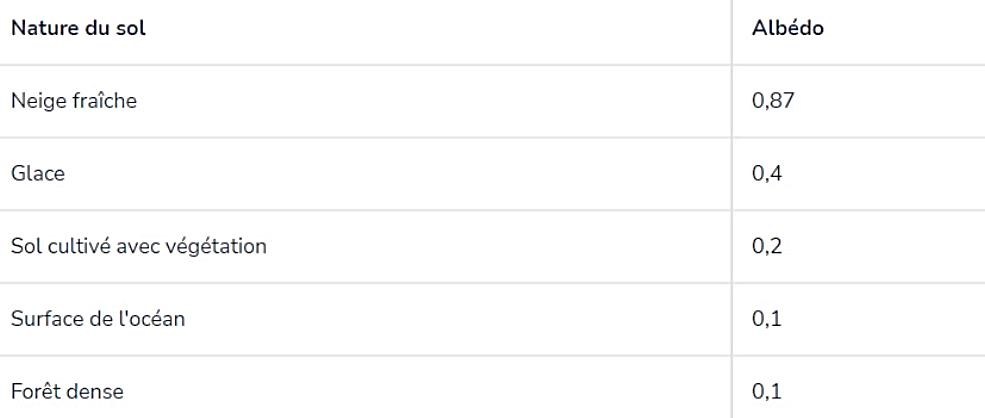
\includegraphics[width=0.8\linewidth]{imgs/p4/albedotable.jpg}
    \caption{Quelques valeurs d'albédo}
\end{figure}
\vspace{1cm}
\begin{rmrq}
L'albédo est une grandeur utilisée principalement en géologie, astronomie et l'étude thermodynamique des planètes, et est un facteur très important dans la dynamique de réchauffement ou de refroidissement planétaire, car il est impliqué dans des \textbf{boucle de rétroaction}\eng{feedback loop}. Prenons l'exemple de la Terre: une grande partie du rayonnement renvoyé par la Terre est du la couleur de la surface de la Terre, notamment le blanche de la neige, principalement dans les régions polaires. Mais avec le réchauffement de la planète, en raison des divers d'autre facteurs, il y a une fonte de ces neiges, ce qui à son tour diminue l'albédo de la Terre, dont le résultat est l'absorption d'une plus grande partie du rayonnement reçu, et donc un réchauffement encore plus rapide, et une fonte des neiges plus rapides, ainsi de suite. Ceci est un exemple d'un \textit{feed-back positif}, où le résultat d'un processus joue le rôle d'accélérateur du processus. Il est intéressant de noter que le cas inverse, est aussi un processus de feed-back positif, C'est-à-dire qu'avec plus de neige, l'albédo augmente, baissant la température moyenne, produisant encore plus de neige, et donc un albédo encore plus important, et ainsi de suite. 
\end{rmrq}


\subsection{L'effet de serre}

\begin{wraptable}{r}{0.3\linewidth}
\begin{rmrq}
\small{Sans effet de serre (ce qui implique notamment : sans vapeur d'eau et sans nuages), et à albédo constant, la température moyenne sur Terre chuterait à −18 °C15. Mais à cette température la glace s'étendrait sur le globe, l'albédo terrestre augmenterait, et la température se stabiliserait vraisemblablement en dessous de −50 °C.}
\end{rmrq}
\end{wraptable}
\begin{quote}
    ``Lorsque le rayonnement solaire atteint l'atmosphère terrestre, une partie (environ $30 \%$) est directement réfléchie, c'est-à-dire renvoyée vers l'espace, par l'air, les nuages blancs et la surface claire de la Terre (on pense évidemment aux régions blanches et glacées comme l'arctique et l'antarctique, mais il ne faut pas en surestimer le rôle : leur position aux pôles fait qu'elles reçoivent peu d'énergie solaire[réf. souhaitée]) ; l'albédo est la mesure de cet effet de miroir. Les rayons incidents qui n'ont pas été réfléchis vers l'espace sont absorbés par l'atmosphère ($20,7 \%$) et la surface terrestre ($51\%$).
    
    Cette dernière partie du rayonnement absorbée par la surface du sol lui apporte de la chaleur qu'elle restitue à son tour, le jour comme la nuit, en direction de l'atmosphère. 
    
    Le transfert de chaleur entre la Terre et l'atmosphère se fait, conformément au deuxième principe de la thermodynamique, du chaud (la terre) vers le froid (l'atmosphère) ; il se fait par convection (réchauffement et humidification de l'air au contact du sol puis ascension de cet air et libération de la chaleur latente de la vapeur d'eau lorsqu'elle se condense en nuages) et sous forme de rayonnements infrarouges lointains (dans la plage $8–13\; \mu m $ principalement, correspondant au « rayonnement du corps noir » pour la température du sol). 
    
    L'effet de serre ne s'intéresse qu'à ces rayonnements, qui seront absorbés en partie par les gaz à effet de serre, ce qui contribue à réchauffer l'atmosphère. Puis dans un troisième temps, cette chaleur contenue par l'atmosphère est ré émise dans toutes les directions ; une partie s'échappe vers l'espace, mais une autre partie retourne vers la Terre et vient en déduction de l'apport de chaleur de la surface vers l'atmosphère, donc s'oppose au refroidissement de la surface1. Il est à noter que l'excès de chaleur généré par les activités humaines, via l’effet de serre, est absorbé à $93\%$ par l'océan, qui atténue ainsi l'augmentation de la température dans l'atmosphère14. L'océan global joue donc un rôle de thermostat planétaire et de contrôle des grands équilibres naturels planétaires. '' (-wikipédia)
\end{quote}


\subsection{Température terrestre moyenne}

la température moyenne du système T-A dépend donc de la différence entre ce que la Terre reçoit, et ce qu'elle renvoi : le bilan thermique Terre-atmosphère. 

\begin{figure}[h]
    \centering
    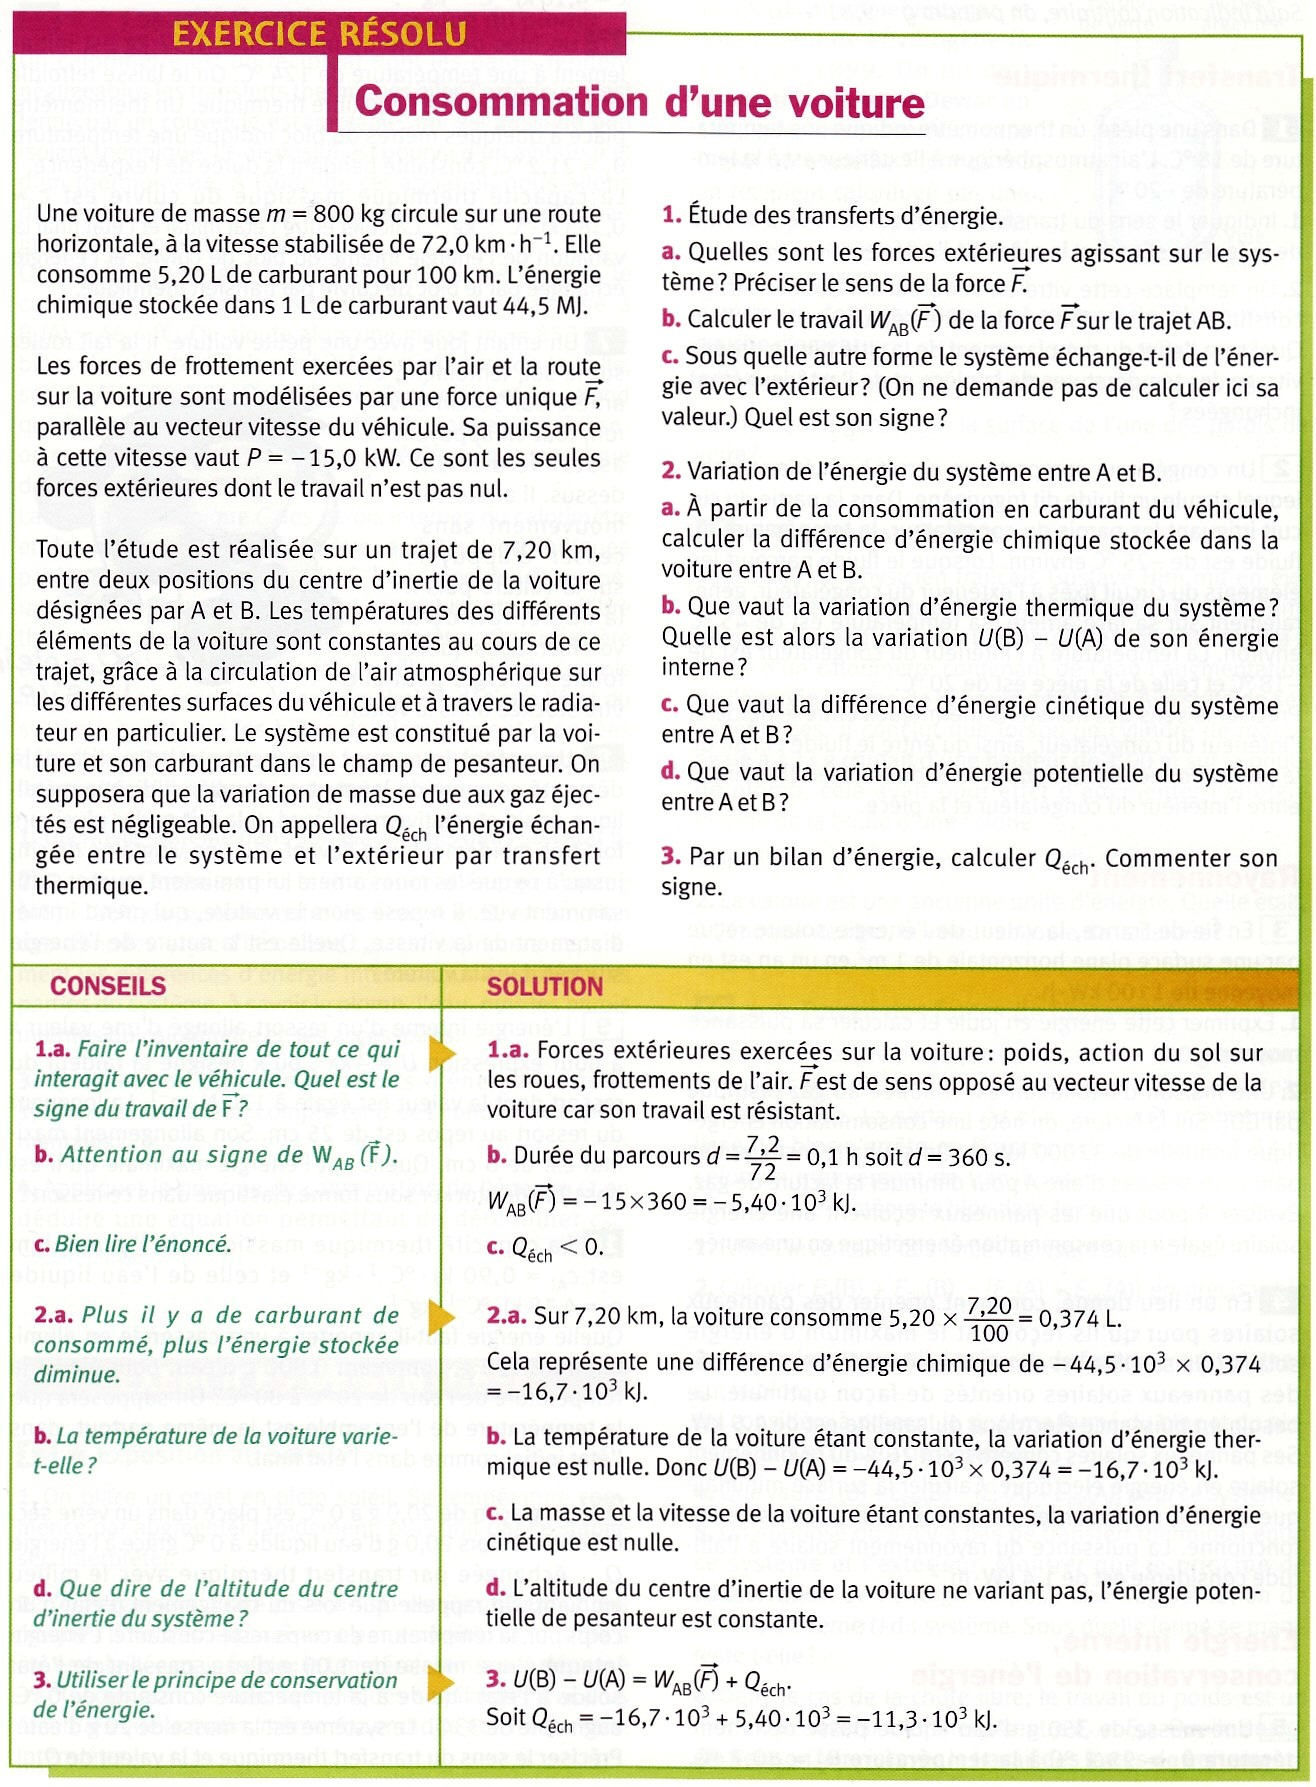
\includegraphics[width=\linewidth]{imgs/p4/xo1.jpg}
\end{figure}

\begin{figure}[h]
    \centering
    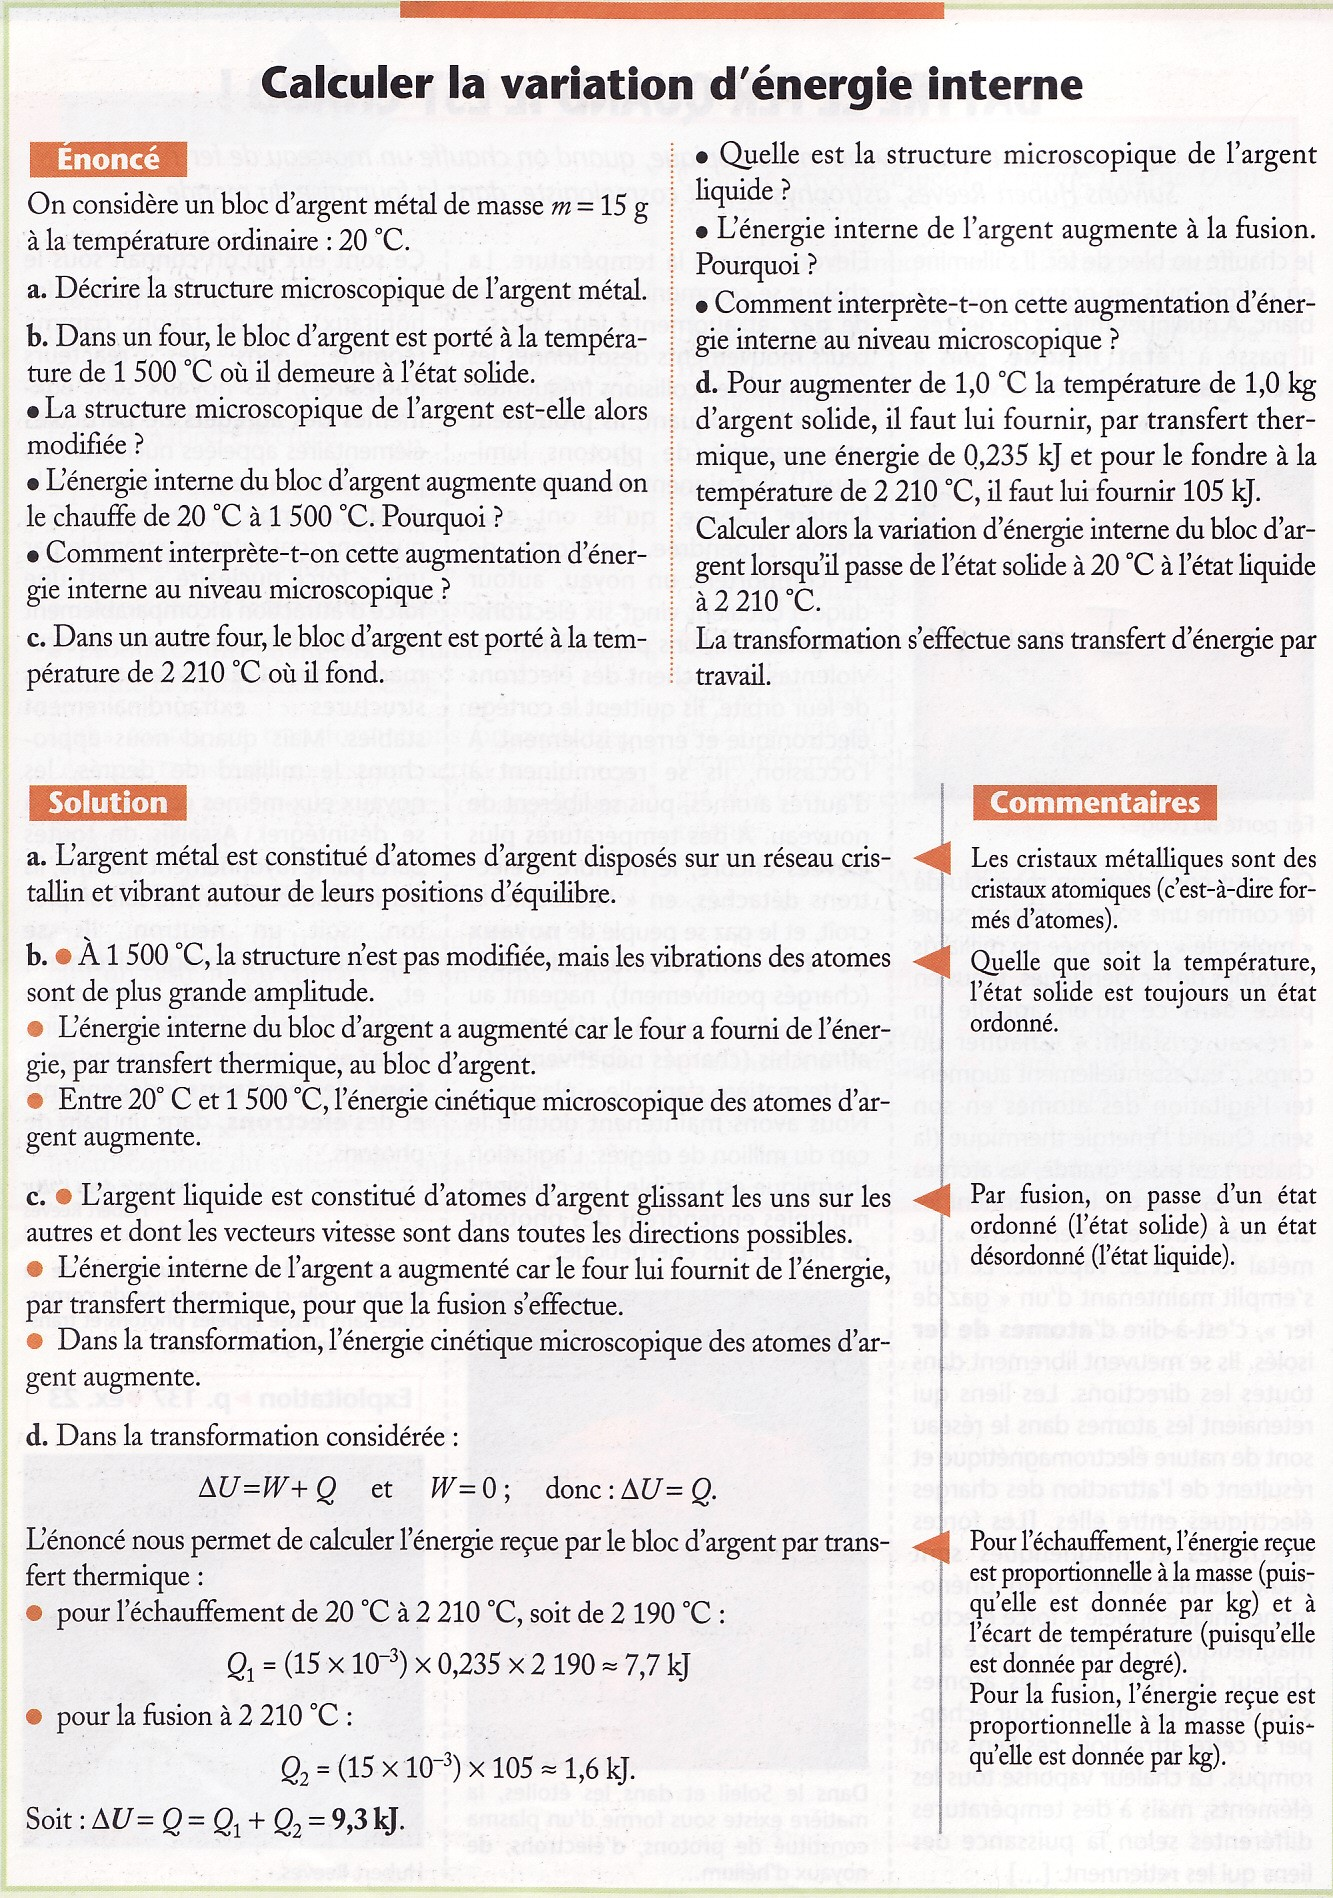
\includegraphics[width=\linewidth]{imgs/p4/xo2.jpg}
\end{figure}


\end{document}